\section{Nonlinear bowl contact under position control}
\label{sec:gap-first-bowl}
We test a soft, tapered nonbox solid falling under gravity into a known rigid
hemispherical bowl (radius 90\,mm), followed by a position-controlled interaction.
The model uses compressible Neo--Hookean tetrahedral mechanics, material-surface
quadrature, penalty contact and regularized friction. It is a bounded nonlinear
contact approximation, not the exact Gaussian force-elimination model.
Geometry, density, damping and gravity are known; Young's modulus and a shared
bowl/tool friction coefficient are uncertain.

\begin{table*}[t]
\centering\small
\begin{tabular}{llrrrrr}
\toprule
Reference & Posterior & Initial motion & After motion & Bowl force & Tool force & Brier \\
 & & \multicolumn{2}{c}{MAP RMS (mm)} & \multicolumn{2}{c}{MAP vector RMS (N)} & \\
\midrule
Matched & Coarse only & 7.59 & 0.02 & 0.001 & 0.001 & 0.000 \\
Matched & Resolution mixture & 8.07 & 0.06 & 0.008 & 0.007 & 0.000 \\
Finer reference & Coarse only & 6.98 & 3.09 & 0.335 & 0.335 & 0.412 \\
Finer reference & Resolution mixture & 3.23 & 0.05 & 0.005 & 0.006 & 0.000 \\
\bottomrule
\end{tabular}
\caption{Bowl study, mean over 16 parameter worlds and two noise replicates.
``After'' uses one selected calibration experiment. Finer-reference results are a
space/time-discretization stress; the secondary mixture contains that reference
model by construction. Full clustered intervals, both fixed controls and conditional
motion/force coverage are retained in the report.}
\label{tab:bowl-gap-results}
\end{table*}
\begin{figure*}[t]
\centering
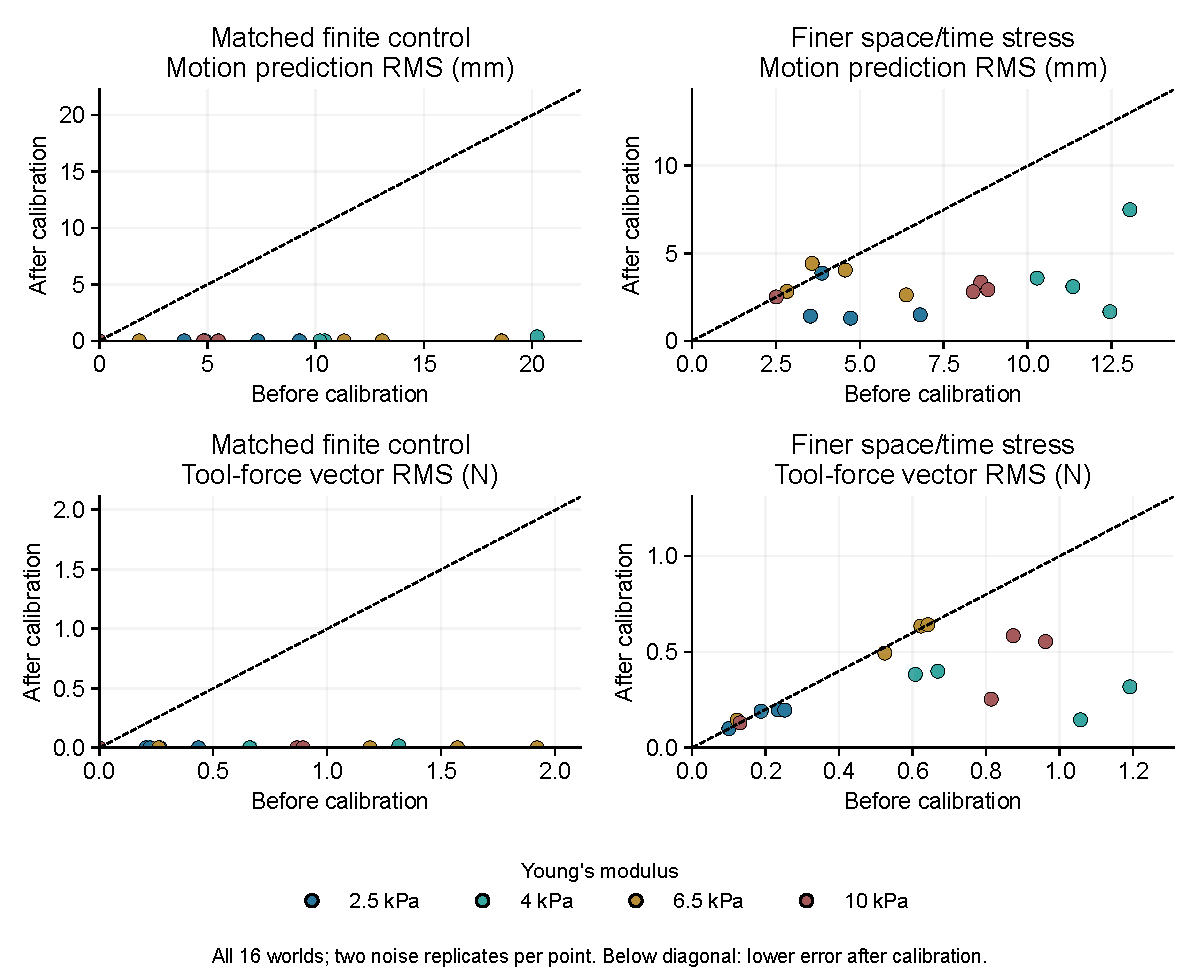
\includegraphics[width=.82\textwidth]{../../output/gap-first-v01/bowl/bowl-all-worlds.pdf}
\caption{All 16 parameter worlds in the controlled finite grid, not 16 distinct
objects. Each point averages two observation-noise replicates. Horizontal and
vertical axes give errors before and after selected calibration; points below
the diagonal improve. Colors identify Young's modulus, with four friction values
per modulus. The matched control and finer space/time stress are shown separately;
these plots do not establish superiority over the best fixed calibration action.}
\label{fig:bowl-all-worlds}
\end{figure*}
\begin{figure*}[t]
\centering
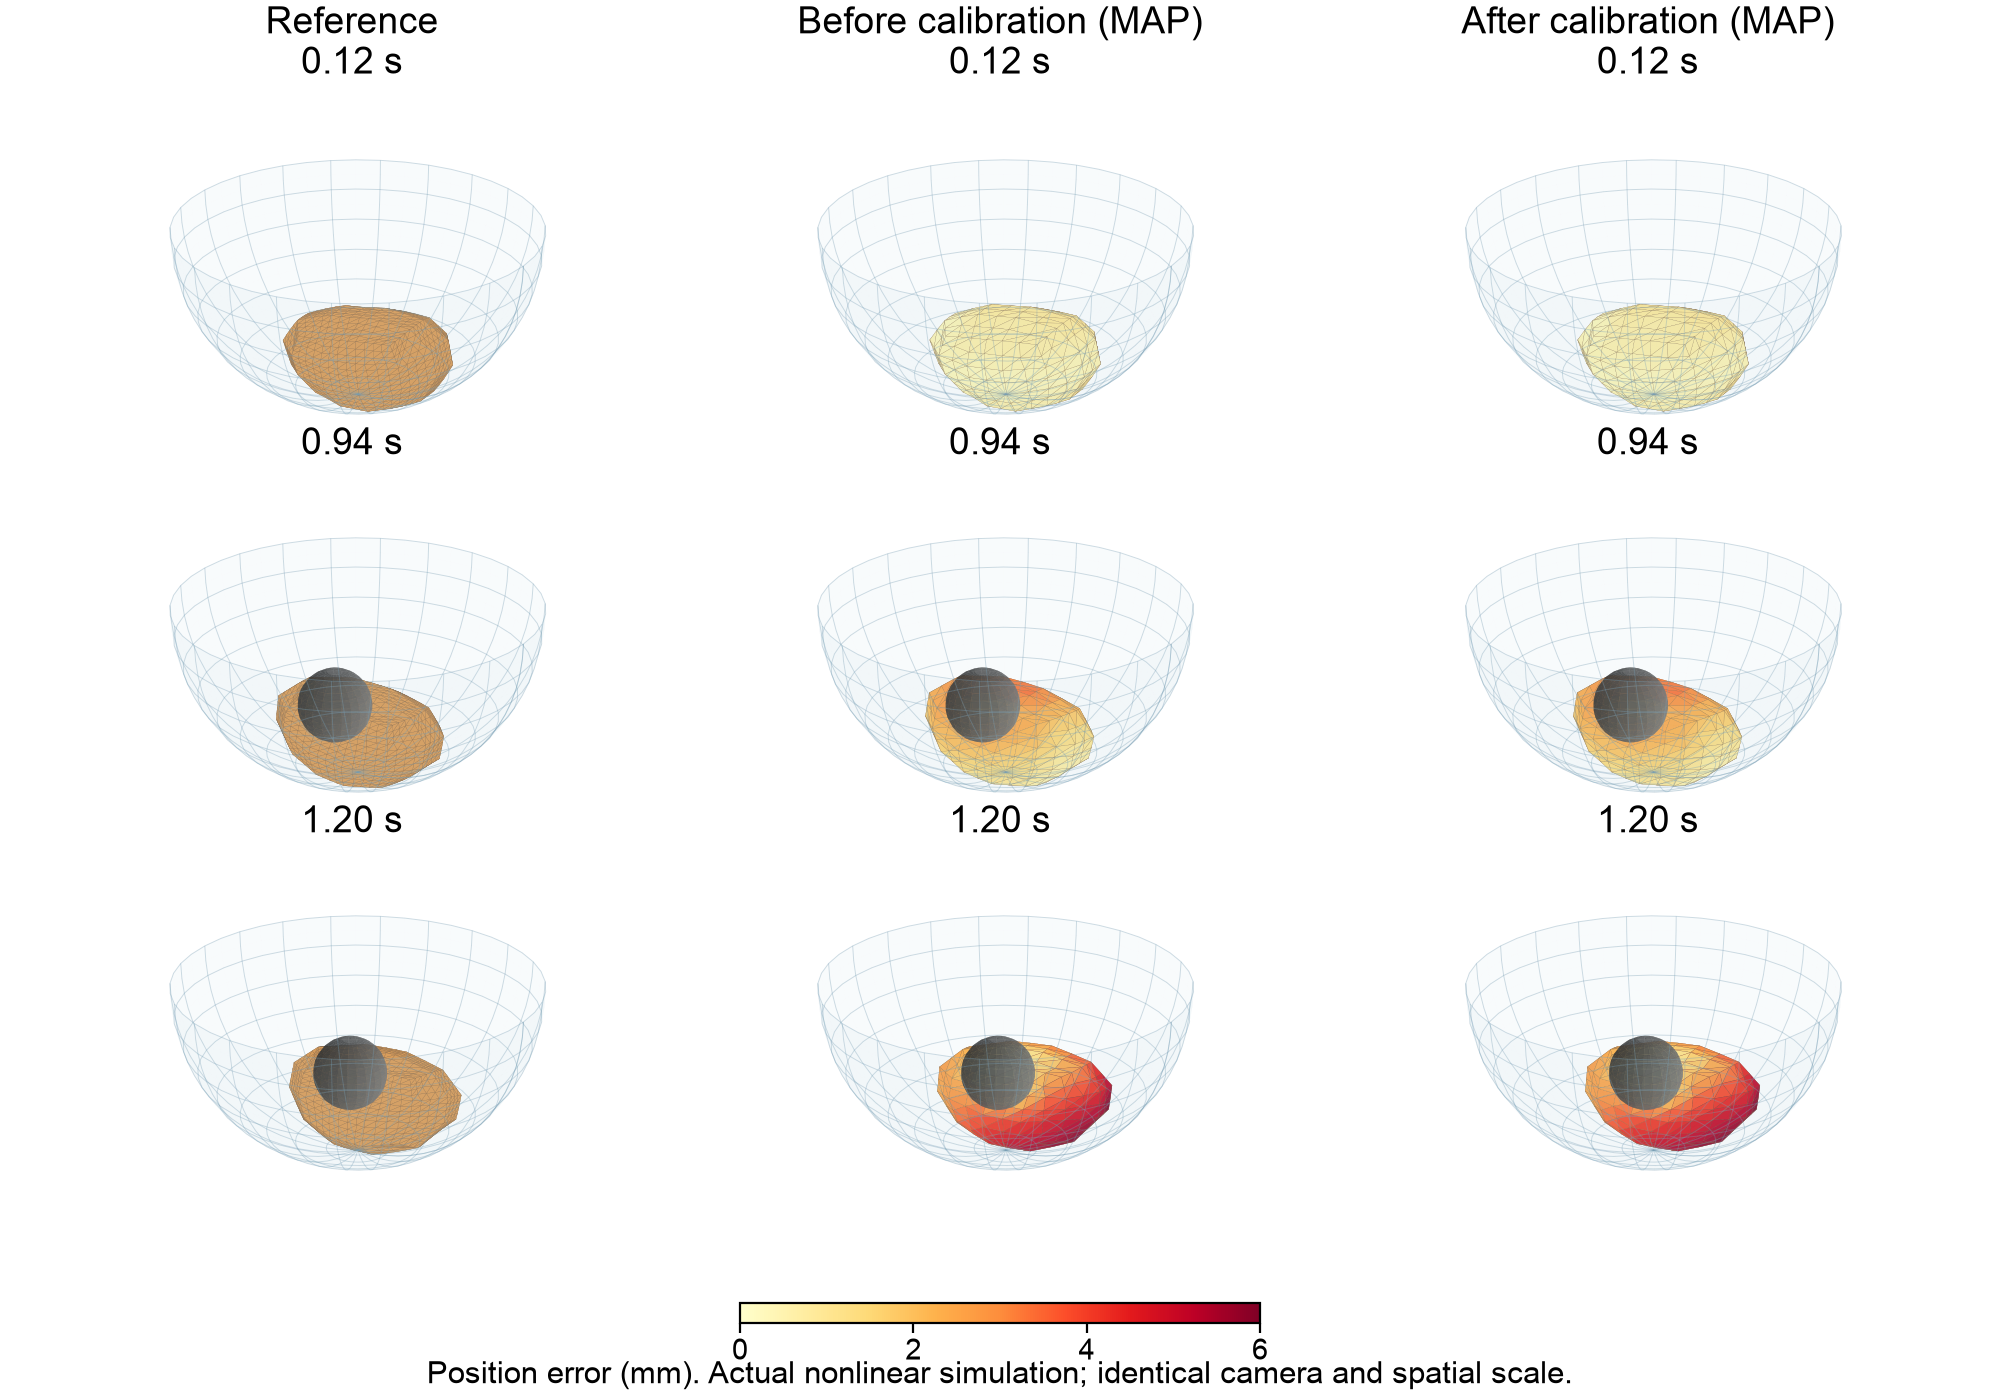
\includegraphics[width=.75\textwidth]{../../output/gap-first-v01/bowl/bowl-refined-case00.png}
\caption{Fixed world 0, noise replicate 0: actual finer-reference geometry and
coarse-only MAP predictions before/after calibration on a separate reset interaction.
All panels use the same camera and true spatial scale; no deformation amplification.
Color encodes position error and saturates at 6\,mm. This is simulated surface
geometry, not a photorealistic-rendering benchmark.}
\label{fig:bowl-fixed-case}
\end{figure*}
\begin{figure*}[t]
\centering
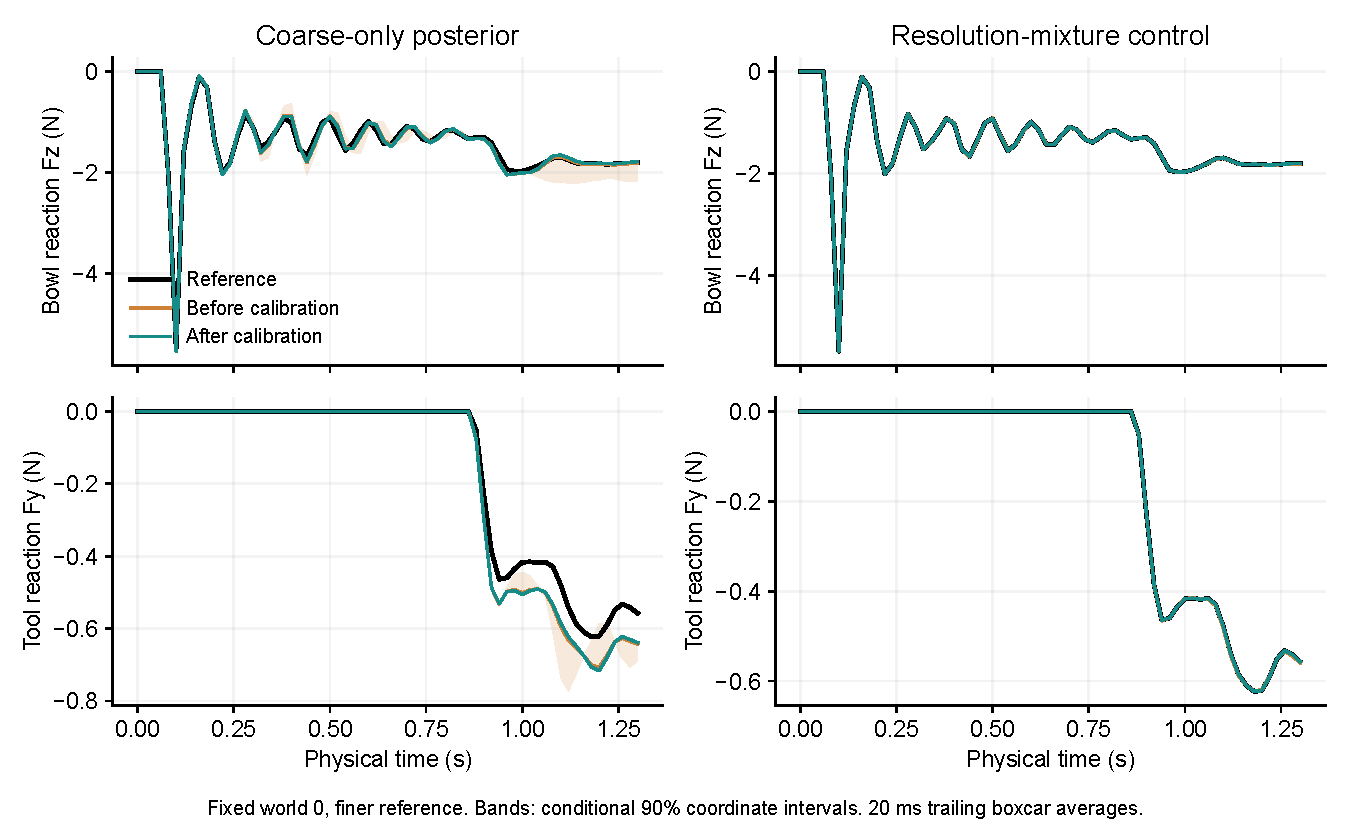
\includegraphics[width=.75\textwidth]{../../output/gap-first-v01/bowl/bowl-force-predictions.pdf}
\caption{Withheld reaction predictions for fixed world 0 of the finer-reference
stress. Only position tracks are observed. Shading gives conditional 90\% coordinate
intervals; the secondary resolution mixture contains the reference by construction.}
\label{fig:bowl-forces}
\end{figure*}
\paragraph{Observation and prediction protocol.}
Sixteen parameter worlds combine four moduli (2.5,4,6.5,10\,kPa) and four friction
coefficients (0.1,0.25,0.45,0.7). We supply four known surface correspondences
projected into an overhead camera, with 0.5\,mm independent coordinate noise.
Initial observations occur at 0.08 and 0.12\,s. Exactly one reset calibration
experiment is selected: a 25\,mm position-controlled push or a 0.2\,rad bowl rotation.
The latter moves the wall tangentially about a fixed spherical center; gravity
does not rotate. New coordinates at 0.94 and 1.2\,s update the posterior. The
separate held-out experiment applies a stronger 45\,mm transverse push after
entering through the open rim. No reaction-force measurements enter inference.

The primary risk is the posterior probability that the deployed MAP model
exceeds 3\,mm point RMS across 64 common material nodes at 1.1,1.2 and 1.3\,s.
This is a fixed-budget calibration comparison, not a proceed-or-acquire policy.
Both fixed actions and the same-evidence MAP predictor are controls. All action
choices and risks are sealed before scoring the selected-world held-out targets.
We evaluate 16 worlds at two discretizations, with two noise replicates each:
64 records, not 64 independent objects. Intervals resample the 16 world clusters.

\paragraph{Qualification and limits.}
Inference uses a 6-cell-per-axis mesh at 25\,$\mu$s; the finer space/time reference
uses 12 cells at 12.5\,$\mu$s, preserving the same piecewise-linear rest geometry.
A 12-cell 25\,$\mu$s development run failed the positive-volume check and is retained
as a numerical failure. The smaller-step soft/stiff controls complete with minimum
Jacobians 0.271/0.372 and sampled penetration 0.172/0.268\,mm. Dense saved-surface
penetration is audited separately. Halving the inference timestep changes the
development target by 0.35\,mm; changing both space and time resolution changes it
by 1.42 and 2.81\,mm. The latter is close to the 3\,mm decision tolerance: this is an
intentional numerical-model stress test, not converged continuum truth.
The open bowl has no rim thickness, continuous collision detection or self-contact.
All 1280 declared marker observations pass the surface/tool/bowl occlusion audit.

\paragraph{Conditional prediction and numerical-model uncertainty.}
Table~\ref{tab:bowl-gap-results} reports the predeclared primary coarse-only posterior
and a secondary 32-hypothesis resolution mixture. The mixture assigns prior 0.5 to
each resolution and the same uniform parameter prior within each. The finer
reference is therefore included by construction; this comparator demonstrates
conditional numerical-model uncertainty, not coverage of arbitrary unknown physics.
The complete report also compares both fixed actions and gives the mixture exactly
the coarse policy's chosen observation, separating model uncertainty from action
selection. Reaction-force errors use 20\,ms trailing boxcar averages accumulated
from every integration step, with bowl and tool scored separately in newtons.

\paragraph{Measured benefit and failure.}
In the matched finite control, selected calibration reduces mean MAP motion error
from 7.588 to 0.023\,mm, but fixed bowl rotation achieves zero MAP error; this does
not establish an advantage over the best fixed experiment. Against the finer
space/time reference, calibration reduces mean error from 6.981 to 3.091\,mm,
while 43.75\% of predictions exceed the 3\,mm tolerance despite a mean predicted
failure probability of only 1.856\%. Conditional 90\% coordinate intervals cover
only 6.14\% of reference coordinates. Fixed rotation has a lower 31.25\% failure
rate. Thus improved motion accuracy does not imply trustworthy uncertainty under
model mismatch. Given exactly the coarse policy's correction observations, the
resolution-mixture control reaches 0.051\,mm mean error and no failures, conditional
on the fine model being included by construction.









An unchanged PhysTwin spring-force kernel was also attempted under the shared
contact/integration adapter. It failed that adapter's positive-tetrahedron-volume
qualification across CPU/GPU and timestep checks. We retain the failure record but
exclude it from accuracy rankings; it is not evidence that the full native PhysTwin
method fails on bowls.
